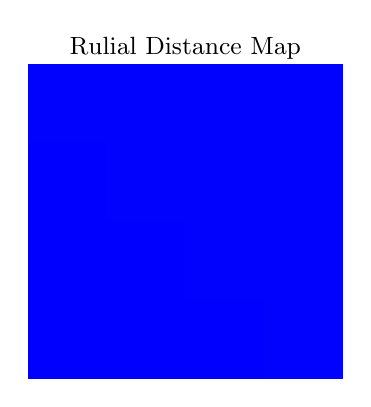
\begin{tikzpicture}
\foreach \x in {0,1,2,3}{
    \foreach \y in {0,1,2,3}{
        \pgfmathsetmacro{\c}{(\x+\y)/6}
        \fill[gray!\c!blue] (\x,\y) rectangle ++(1,1);
    }
}
\node at (2,4.2) {\small Rulial Distance Map};
\end{tikzpicture}